 \documentclass{article}
\usepackage[utf8]{inputenc}
\usepackage[a4paper, total={7in, 10in}]{geometry}
\usepackage{braket}
\usepackage{xcolor}
\usepackage{amsmath}
\usepackage{amssymb}
\usepackage{amsfonts}
\usepackage{graphicx}
\usepackage{svg}
\usepackage{float}
\usepackage{tikz}
\usepackage[ruled,vlined]{algorithm2e}
\usepackage{multicol}
\usepackage[backend=biber,style=alphabetic,sorting=ynt]{biblatex}
\usepackage{xcolor}
%\addbibresource{sample.bib} %Import the bibliography file

\newcommand{\commentt}[1]{\textcolor{blue}{ \textbf{[COMMENT]} #1}}
\newcommand{\ctt}[1]{\commentt{#1}}
\newcommand{\prb}[1]{ \mathbf{Pr} \left[ {#1} \right]}
\newcommand{\onotation}[1]{\(\mathcal{O} \left( {#1}  \right) \)}
\newcommand{\ona}[1]{\onotation{#1}}
\newcommand{\PSI}{{\ket{\psi}}}
\newcommand{\LESn}{\ket{\psi_n}}
\newcommand{\LESa}{\ket{\phi_n}}
\newcommand{\LESs}{\frac{1}{\sqrt{n}}\sum_{i}{\ket{\left(0^{i}10^{n-i}\right)^{n}}}}
\newcommand{\Hn}{\mathcal{H}_{n}}
\newcommand{\Ep}{\frac{1}{\sqrt{2^n}}\sum^{2^n}_{x}{ \ket{xx}}}
\newcommand{\HON}{\ket{\psi_{\text{honest}}}}
\newcommand{\Lemma}{\paragraph{Lemma.}}


\setlength{\columnsep}{0.6cm}

\newcommand{\Gz}{ G_{z}^{\delta} } 

\begin{document}

\title{Quantum LTC With Positive Rate}
\author{David Ponarovsky}
\maketitle
\begin{multicols*}{2}
\newcommand{ \Hw }{ \delta\Delta -\Delta^{\frac{1}{2}-\varepsilon}/\delta  }
	\newcommand{ \Nw }{ \Delta^{\frac{3}{2}-\varepsilon}} 
	  \newcommand{ \Gu } { \Gamma^{\cup} }
	  \newcommand{ \Guq } { \Gamma^{\cup, \square} }

    	\newcommand{ \Gsa } {\Gamma_{\square_{1}} }
	\newcommand{ \Gsb } {\Gamma_{\square_{2}} }
        \newcommand{ \Aa } { C_{A_{1}}}  
	\newcommand{ \Ab } { C_{A_{2}}}
	\newcommand{ \Ac } { C_{A_{3}}}
	\newcommand{ \Aab } { \Aa \otimes \Ab } 
	\newcommand{ \Aac } { \Aa \otimes \Ac }
	\newcommand{ \Aabc } { \Aa \otimes \Ab \otimes \Ac }
	\newcommand{ \Aabp } { \Aa^{\perp} \otimes \Ab^{\perp} } 
	\newcommand{ \Aacp } { \Aa^{\perp} \otimes \Ac^{\perp} }
	\newcommand{ \Aabcp } { \Aa^{\perp} \otimes \Ab^{\perp} \otimes \Ac^{\perp} }
	\newcommand{ \Aabpp } { \left( \Aabp \right)^\perp } 
	\newcommand{ \Aacpp } { \left( \Aacp \right)^\perp }
	\newcommand{ \Aabcpp } { \left( \Aabcp \right)^\perp }
	\newcommand{ \YY } {  y_{1}y_{2}^{\top} }
	\newcommand{ \ZZ } {  z_{1}z_{2}^{\top} } 
	\newcommand{ \TT } { \tilde{\tau} } 


  \paragraph{preamble.} preamble.  
  \begin{figure}[H]
            %\label{fig:square}
            \begin{center}
            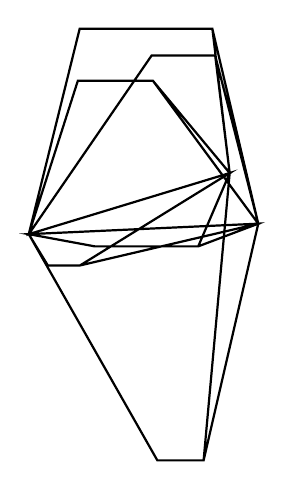
\begin{tikzpicture}
            \draw[thick](0,0)(0,0)  -- (0.6462160369442271, 2.6082073058060677) -- (2.3314158563856244, 2.6082073058060677) -- (2.5513188392523314,0.7760687289086533) -- (0,0) -- (0,0)  -- (0.24250198074345053, -0.39762073842304935) -- (0.650215868101282, -0.39762073842304935) -- (2.5513188392523314,0.7760687289086533) -- (0,0) -- 
(0,0)  -- (0.6462160369442271, 2.6082073058060677) -- (2.3314158563856244, 2.6082073058060677) -- (2.5513188392523314,0.7760687289086533) -- (0,0) -- (0,0)  -- (1.6328770247710755, -2.87321762704413) -- (2.220228457347136, -2.87321762704413) -- (2.5513188392523314,0.7760687289086533) -- (0,0) -- 
(0,0)  -- (0.6462160369442271, 2.6082073058060677) -- (2.3314158563856244, 2.6082073058060677) -- (2.5513188392523314,0.7760687289086533) -- (0,0) -- (0,0)  -- (0.8382782192225489, -0.15511475587797907) -- (2.1521784027347097, -0.15511475587797907) -- (2.5513188392523314,0.7760687289086533) -- (0,0) -- 
(0,0)  -- (0.6229938297788458, 1.9480275184614915) -- (1.5764110326641958, 1.9480275184614915) -- (2.5513188392523314,0.7760687289086533) -- (0,0) -- (0,0)  -- (0.24250198074345053, -0.39762073842304935) -- (0.650215868101282, -0.39762073842304935) -- (2.5513188392523314,0.7760687289086533) -- (0,0) -- 
(0,0)  -- (0.6229938297788458, 1.9480275184614915) -- (1.5764110326641958, 1.9480275184614915) -- (2.5513188392523314,0.7760687289086533) -- (0,0) -- (0,0)  -- (1.6328770247710755, -2.87321762704413) -- (2.220228457347136, -2.87321762704413) -- (2.5513188392523314,0.7760687289086533) -- (0,0) -- 
(0,0)  -- (0.6229938297788458, 1.9480275184614915) -- (1.5764110326641958, 1.9480275184614915) -- (2.5513188392523314,0.7760687289086533) -- (0,0) -- (0,0)  -- (0.8382782192225489, -0.15511475587797907) -- (2.1521784027347097, -0.15511475587797907) -- (2.5513188392523314,0.7760687289086533) -- (0,0) -- 
(0,0)  -- (1.5605553666921814, 2.2693388449923235) -- (2.3670871208395656, 2.2693388449923235) -- (2.5513188392523314,0.7760687289086533) -- (0,0) -- (0,0)  -- (0.24250198074345053, -0.39762073842304935) -- (0.650215868101282, -0.39762073842304935) -- (2.5513188392523314,0.7760687289086533) -- (0,0) -- 
(0,0)  -- (1.5605553666921814, 2.2693388449923235) -- (2.3670871208395656, 2.2693388449923235) -- (2.5513188392523314,0.7760687289086533) -- (0,0) -- (0,0)  -- (1.6328770247710755, -2.87321762704413) -- (2.220228457347136, -2.87321762704413) -- (2.5513188392523314,0.7760687289086533) -- (0,0) -- 
(0,0)  -- (1.5605553666921814, 2.2693388449923235) -- (2.3670871208395656, 2.2693388449923235) -- (2.5513188392523314,0.7760687289086533) -- (0,0) -- (0,0)  -- (0.8382782192225489, -0.15511475587797907) -- (2.1521784027347097, -0.15511475587797907) -- (2.5513188392523314,0.7760687289086533) -- (0,0) -- 
(0,0)  -- (0.6462160369442271, 2.6082073058060677) -- (2.3314158563856244, 2.6082073058060677) -- (2.914446251749685,0.13300268092373915) -- (0,0) -- (0,0)  -- (0.24250198074345053, -0.39762073842304935) -- (0.650215868101282, -0.39762073842304935) -- (2.914446251749685,0.13300268092373915) -- (0,0) -- 
(0,0)  -- (0.6462160369442271, 2.6082073058060677) -- (2.3314158563856244, 2.6082073058060677) -- (2.914446251749685,0.13300268092373915) -- (0,0) -- (0,0)  -- (1.6328770247710755, -2.87321762704413) -- (2.220228457347136, -2.87321762704413) -- (2.914446251749685,0.13300268092373915) -- (0,0) -- 
(0,0)  -- (0.6462160369442271, 2.6082073058060677) -- (2.3314158563856244, 2.6082073058060677) -- (2.914446251749685,0.13300268092373915) -- (0,0) -- (0,0)  -- (0.8382782192225489, -0.15511475587797907) -- (2.1521784027347097, -0.15511475587797907) -- (2.914446251749685,0.13300268092373915) -- (0,0) -- 
(0,0)  -- (0.6229938297788458, 1.9480275184614915) -- (1.5764110326641958, 1.9480275184614915) -- (2.914446251749685,0.13300268092373915) -- (0,0) -- (0,0)  -- (0.24250198074345053, -0.39762073842304935) -- (0.650215868101282, -0.39762073842304935) -- (2.914446251749685,0.13300268092373915) -- (0,0) -- 
(0,0)  -- (0.6229938297788458, 1.9480275184614915) -- (1.5764110326641958, 1.9480275184614915) -- (2.914446251749685,0.13300268092373915) -- (0,0) -- (0,0)  -- (1.6328770247710755, -2.87321762704413) -- (2.220228457347136, -2.87321762704413) -- (2.914446251749685,0.13300268092373915) -- (0,0) -- 
(0,0)  -- (0.6229938297788458, 1.9480275184614915) -- (1.5764110326641958, 1.9480275184614915) -- (2.914446251749685,0.13300268092373915) -- (0,0) -- (0,0)  -- (0.8382782192225489, -0.15511475587797907) -- (2.1521784027347097, -0.15511475587797907) -- (2.914446251749685,0.13300268092373915) -- (0,0) -- 
(0,0)  -- (1.5605553666921814, 2.2693388449923235) -- (2.3670871208395656, 2.2693388449923235) -- (2.914446251749685,0.13300268092373915) -- (0,0) -- (0,0)  -- (0.24250198074345053, -0.39762073842304935) -- (0.650215868101282, -0.39762073842304935) -- (2.914446251749685,0.13300268092373915) -- (0,0) -- 
(0,0)  -- (1.5605553666921814, 2.2693388449923235) -- (2.3670871208395656, 2.2693388449923235) -- (2.914446251749685,0.13300268092373915) -- (0,0) -- (0,0)  -- (1.6328770247710755, -2.87321762704413) -- (2.220228457347136, -2.87321762704413) -- (2.914446251749685,0.13300268092373915) -- (0,0) -- 
(0,0)  -- (1.5605553666921814, 2.2693388449923235) -- (2.3670871208395656, 2.2693388449923235) -- (2.914446251749685,0.13300268092373915) -- (0,0) -- (0,0)  -- (0.8382782192225489, -0.15511475587797907) -- (2.1521784027347097, -0.15511475587797907) -- (2.914446251749685,0.13300268092373915) -- (0,0) -- 
(0,0);
            \end{tikzpicture}
            \end{center}
            \caption{Square of the complex, with edges $(g,ag), (agb, gb) \in E_A,
            (g,gb), (agb, ag) \in E_B.$ \label{fig:square}
            }
            \end{figure}\n \begin{figure}[H]
            %\label{fig:square}
            \begin{center}
            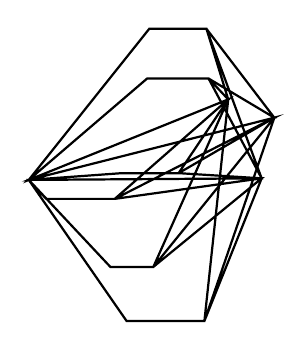
\begin{tikzpicture}
            \draw[thick](0,0)(0,0)  -- (1.50339017776742, 1.2879398106260271) -- (2.2830492986201474, 1.2879398106260271) -- (3.118276860968746,0.7901602219111401) -- (0,0) -- (0,0)  -- (1.0363177367671548, -1.1052498838624407) -- (1.5816764721473016, -1.1052498838624407) -- (3.118276860968746,0.7901602219111401) -- (0,0) -- 
(0,0)  -- (1.50339017776742, 1.2879398106260271) -- (2.2830492986201474, 1.2879398106260271) -- (3.118276860968746,0.7901602219111401) -- (0,0) -- (0,0)  -- (1.2422542944565704, -1.7919543570124992) -- (2.230329194438278, -1.7919543570124992) -- (3.118276860968746,0.7901602219111401) -- (0,0) -- 
(0,0)  -- (1.50339017776742, 1.2879398106260271) -- (2.2830492986201474, 1.2879398106260271) -- (3.118276860968746,0.7901602219111401) -- (0,0) -- (0,0)  -- (0.22116338529091673, -0.2407527993224713) -- (1.0919440260711493, -0.2407527993224713) -- (3.118276860968746,0.7901602219111401) -- (0,0) -- 
(0,0)  -- (1.1818533480534776, 0.08585572492953497) -- (1.9028289831137613, 0.08585572492953497) -- (3.118276860968746,0.7901602219111401) -- (0,0) -- (0,0)  -- (1.0363177367671548, -1.1052498838624407) -- (1.5816764721473016, -1.1052498838624407) -- (3.118276860968746,0.7901602219111401) -- (0,0) -- 
(0,0)  -- (1.1818533480534776, 0.08585572492953497) -- (1.9028289831137613, 0.08585572492953497) -- (3.118276860968746,0.7901602219111401) -- (0,0) -- (0,0)  -- (1.2422542944565704, -1.7919543570124992) -- (2.230329194438278, -1.7919543570124992) -- (3.118276860968746,0.7901602219111401) -- (0,0) -- 
(0,0)  -- (1.1818533480534776, 0.08585572492953497) -- (1.9028289831137613, 0.08585572492953497) -- (3.118276860968746,0.7901602219111401) -- (0,0) -- (0,0)  -- (0.22116338529091673, -0.2407527993224713) -- (1.0919440260711493, -0.2407527993224713) -- (3.118276860968746,0.7901602219111401) -- (0,0) -- 
(0,0)  -- (1.5302934455694779, 1.9193325038427265) -- (2.2563962472813253, 1.9193325038427265) -- (3.118276860968746,0.7901602219111401) -- (0,0) -- (0,0)  -- (1.0363177367671548, -1.1052498838624407) -- (1.5816764721473016, -1.1052498838624407) -- (3.118276860968746,0.7901602219111401) -- (0,0) -- 
(0,0)  -- (1.5302934455694779, 1.9193325038427265) -- (2.2563962472813253, 1.9193325038427265) -- (3.118276860968746,0.7901602219111401) -- (0,0) -- (0,0)  -- (1.2422542944565704, -1.7919543570124992) -- (2.230329194438278, -1.7919543570124992) -- (3.118276860968746,0.7901602219111401) -- (0,0) -- 
(0,0)  -- (1.5302934455694779, 1.9193325038427265) -- (2.2563962472813253, 1.9193325038427265) -- (3.118276860968746,0.7901602219111401) -- (0,0) -- (0,0)  -- (0.22116338529091673, -0.2407527993224713) -- (1.0919440260711493, -0.2407527993224713) -- (3.118276860968746,0.7901602219111401) -- (0,0) -- 
(0,0)  -- (1.50339017776742, 1.2879398106260271) -- (2.2830492986201474, 1.2879398106260271) -- (2.532817570315622,1.0225331215726963) -- (0,0) -- (0,0)  -- (1.0363177367671548, -1.1052498838624407) -- (1.5816764721473016, -1.1052498838624407) -- (2.532817570315622,1.0225331215726963) -- (0,0) -- 
(0,0)  -- (1.50339017776742, 1.2879398106260271) -- (2.2830492986201474, 1.2879398106260271) -- (2.532817570315622,1.0225331215726963) -- (0,0) -- (0,0)  -- (1.2422542944565704, -1.7919543570124992) -- (2.230329194438278, -1.7919543570124992) -- (2.532817570315622,1.0225331215726963) -- (0,0) -- 
(0,0)  -- (1.50339017776742, 1.2879398106260271) -- (2.2830492986201474, 1.2879398106260271) -- (2.532817570315622,1.0225331215726963) -- (0,0) -- (0,0)  -- (0.22116338529091673, -0.2407527993224713) -- (1.0919440260711493, -0.2407527993224713) -- (2.532817570315622,1.0225331215726963) -- (0,0) -- 
(0,0)  -- (1.1818533480534776, 0.08585572492953497) -- (1.9028289831137613, 0.08585572492953497) -- (2.532817570315622,1.0225331215726963) -- (0,0) -- (0,0)  -- (1.0363177367671548, -1.1052498838624407) -- (1.5816764721473016, -1.1052498838624407) -- (2.532817570315622,1.0225331215726963) -- (0,0) -- 
(0,0)  -- (1.1818533480534776, 0.08585572492953497) -- (1.9028289831137613, 0.08585572492953497) -- (2.532817570315622,1.0225331215726963) -- (0,0) -- (0,0)  -- (1.2422542944565704, -1.7919543570124992) -- (2.230329194438278, -1.7919543570124992) -- (2.532817570315622,1.0225331215726963) -- (0,0) -- 
(0,0)  -- (1.1818533480534776, 0.08585572492953497) -- (1.9028289831137613, 0.08585572492953497) -- (2.532817570315622,1.0225331215726963) -- (0,0) -- (0,0)  -- (0.22116338529091673, -0.2407527993224713) -- (1.0919440260711493, -0.2407527993224713) -- (2.532817570315622,1.0225331215726963) -- (0,0) -- 
(0,0)  -- (1.5302934455694779, 1.9193325038427265) -- (2.2563962472813253, 1.9193325038427265) -- (2.532817570315622,1.0225331215726963) -- (0,0) -- (0,0)  -- (1.0363177367671548, -1.1052498838624407) -- (1.5816764721473016, -1.1052498838624407) -- (2.532817570315622,1.0225331215726963) -- (0,0) -- 
(0,0)  -- (1.5302934455694779, 1.9193325038427265) -- (2.2563962472813253, 1.9193325038427265) -- (2.532817570315622,1.0225331215726963) -- (0,0) -- (0,0)  -- (1.2422542944565704, -1.7919543570124992) -- (2.230329194438278, -1.7919543570124992) -- (2.532817570315622,1.0225331215726963) -- (0,0) -- 
(0,0)  -- (1.5302934455694779, 1.9193325038427265) -- (2.2563962472813253, 1.9193325038427265) -- (2.532817570315622,1.0225331215726963) -- (0,0) -- (0,0)  -- (0.22116338529091673, -0.2407527993224713) -- (1.0919440260711493, -0.2407527993224713) -- (2.532817570315622,1.0225331215726963) -- (0,0) -- 
(0,0)  -- (1.50339017776742, 1.2879398106260271) -- (2.2830492986201474, 1.2879398106260271) -- (2.957292734174953,0.019965407389273614) -- (0,0) -- (0,0)  -- (1.0363177367671548, -1.1052498838624407) -- (1.5816764721473016, -1.1052498838624407) -- (2.957292734174953,0.019965407389273614) -- (0,0) -- 
(0,0)  -- (1.50339017776742, 1.2879398106260271) -- (2.2830492986201474, 1.2879398106260271) -- (2.957292734174953,0.019965407389273614) -- (0,0) -- (0,0)  -- (1.2422542944565704, -1.7919543570124992) -- (2.230329194438278, -1.7919543570124992) -- (2.957292734174953,0.019965407389273614) -- (0,0) -- 
(0,0)  -- (1.50339017776742, 1.2879398106260271) -- (2.2830492986201474, 1.2879398106260271) -- (2.957292734174953,0.019965407389273614) -- (0,0) -- (0,0)  -- (0.22116338529091673, -0.2407527993224713) -- (1.0919440260711493, -0.2407527993224713) -- (2.957292734174953,0.019965407389273614) -- (0,0) -- 
(0,0)  -- (1.1818533480534776, 0.08585572492953497) -- (1.9028289831137613, 0.08585572492953497) -- (2.957292734174953,0.019965407389273614) -- (0,0) -- (0,0)  -- (1.0363177367671548, -1.1052498838624407) -- (1.5816764721473016, -1.1052498838624407) -- (2.957292734174953,0.019965407389273614) -- (0,0) -- 
(0,0)  -- (1.1818533480534776, 0.08585572492953497) -- (1.9028289831137613, 0.08585572492953497) -- (2.957292734174953,0.019965407389273614) -- (0,0) -- (0,0)  -- (1.2422542944565704, -1.7919543570124992) -- (2.230329194438278, -1.7919543570124992) -- (2.957292734174953,0.019965407389273614) -- (0,0) -- 
(0,0)  -- (1.1818533480534776, 0.08585572492953497) -- (1.9028289831137613, 0.08585572492953497) -- (2.957292734174953,0.019965407389273614) -- (0,0) -- (0,0)  -- (0.22116338529091673, -0.2407527993224713) -- (1.0919440260711493, -0.2407527993224713) -- (2.957292734174953,0.019965407389273614) -- (0,0) -- 
(0,0)  -- (1.5302934455694779, 1.9193325038427265) -- (2.2563962472813253, 1.9193325038427265) -- (2.957292734174953,0.019965407389273614) -- (0,0) -- (0,0)  -- (1.0363177367671548, -1.1052498838624407) -- (1.5816764721473016, -1.1052498838624407) -- (2.957292734174953,0.019965407389273614) -- (0,0) -- 
(0,0)  -- (1.5302934455694779, 1.9193325038427265) -- (2.2563962472813253, 1.9193325038427265) -- (2.957292734174953,0.019965407389273614) -- (0,0) -- (0,0)  -- (1.2422542944565704, -1.7919543570124992) -- (2.230329194438278, -1.7919543570124992) -- (2.957292734174953,0.019965407389273614) -- (0,0) -- 
(0,0)  -- (1.5302934455694779, 1.9193325038427265) -- (2.2563962472813253, 1.9193325038427265) -- (2.957292734174953,0.019965407389273614) -- (0,0) -- (0,0)  -- (0.22116338529091673, -0.2407527993224713) -- (1.0919440260711493, -0.2407527993224713) -- (2.957292734174953,0.019965407389273614) -- (0,0) -- 
(0,0);
            \end{tikzpicture}
            \end{center}
            \caption{Square of the complex, with edges $(g,ag), (agb, gb) \in E_A,
            (g,gb), (agb, ag) \in E_B.$ \label{fig:square}
            }
            \end{figure}\n \begin{figure}[H]
            %\label{fig:square}
            \begin{center}
            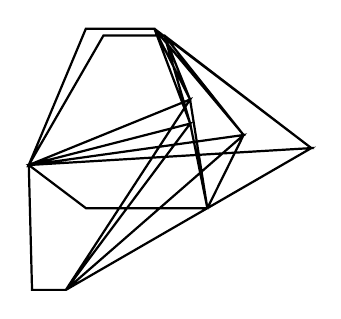
\begin{tikzpicture}
            \draw[thick](0,0)(0,0)  -- (0.7244919848591642, 1.7302900694513697) -- (1.5961049434090502, 1.7302900694513697) -- (2.0482505993756472,0.8320713035453493) -- (0,0) -- (0,0)  -- (0.7264578559047401, -0.5485754362363084) -- (2.2679334227336136, -0.5485754362363084) -- (2.0482505993756472,0.8320713035453493) -- (0,0) -- 
(0,0)  -- (0.7244919848591642, 1.7302900694513697) -- (1.5961049434090502, 1.7302900694513697) -- (2.0482505993756472,0.8320713035453493) -- (0,0) -- (0,0)  -- (0.04135353971655298, -1.5856221480482224) -- (0.4712783964991998, -1.5856221480482224) -- (2.0482505993756472,0.8320713035453493) -- (0,0) -- 
(0,0)  -- (0.9483977642895416, 1.6447191017559823) -- (1.721488282704015, 1.6447191017559823) -- (2.0482505993756472,0.8320713035453493) -- (0,0) -- (0,0)  -- (0.7264578559047401, -0.5485754362363084) -- (2.2679334227336136, -0.5485754362363084) -- (2.0482505993756472,0.8320713035453493) -- (0,0) -- 
(0,0)  -- (0.9483977642895416, 1.6447191017559823) -- (1.721488282704015, 1.6447191017559823) -- (2.0482505993756472,0.8320713035453493) -- (0,0) -- (0,0)  -- (0.04135353971655298, -1.5856221480482224) -- (0.4712783964991998, -1.5856221480482224) -- (2.0482505993756472,0.8320713035453493) -- (0,0) -- 
(0,0)  -- (0.7244919848591642, 1.7302900694513697) -- (1.5961049434090502, 1.7302900694513697) -- (3.588521220309592,0.21508464795123086) -- (0,0) -- (0,0)  -- (0.7264578559047401, -0.5485754362363084) -- (2.2679334227336136, -0.5485754362363084) -- (3.588521220309592,0.21508464795123086) -- (0,0) -- 
(0,0)  -- (0.7244919848591642, 1.7302900694513697) -- (1.5961049434090502, 1.7302900694513697) -- (3.588521220309592,0.21508464795123086) -- (0,0) -- (0,0)  -- (0.04135353971655298, -1.5856221480482224) -- (0.4712783964991998, -1.5856221480482224) -- (3.588521220309592,0.21508464795123086) -- (0,0) -- 
(0,0)  -- (0.9483977642895416, 1.6447191017559823) -- (1.721488282704015, 1.6447191017559823) -- (3.588521220309592,0.21508464795123086) -- (0,0) -- (0,0)  -- (0.7264578559047401, -0.5485754362363084) -- (2.2679334227336136, -0.5485754362363084) -- (3.588521220309592,0.21508464795123086) -- (0,0) -- 
(0,0)  -- (0.9483977642895416, 1.6447191017559823) -- (1.721488282704015, 1.6447191017559823) -- (3.588521220309592,0.21508464795123086) -- (0,0) -- (0,0)  -- (0.04135353971655298, -1.5856221480482224) -- (0.4712783964991998, -1.5856221480482224) -- (3.588521220309592,0.21508464795123086) -- (0,0) -- 
(0,0)  -- (0.7244919848591642, 1.7302900694513697) -- (1.5961049434090502, 1.7302900694513697) -- (2.0500107943958237,0.5262953527498213) -- (0,0) -- (0,0)  -- (0.7264578559047401, -0.5485754362363084) -- (2.2679334227336136, -0.5485754362363084) -- (2.0500107943958237,0.5262953527498213) -- (0,0) -- 
(0,0)  -- (0.7244919848591642, 1.7302900694513697) -- (1.5961049434090502, 1.7302900694513697) -- (2.0500107943958237,0.5262953527498213) -- (0,0) -- (0,0)  -- (0.04135353971655298, -1.5856221480482224) -- (0.4712783964991998, -1.5856221480482224) -- (2.0500107943958237,0.5262953527498213) -- (0,0) -- 
(0,0)  -- (0.9483977642895416, 1.6447191017559823) -- (1.721488282704015, 1.6447191017559823) -- (2.0500107943958237,0.5262953527498213) -- (0,0) -- (0,0)  -- (0.7264578559047401, -0.5485754362363084) -- (2.2679334227336136, -0.5485754362363084) -- (2.0500107943958237,0.5262953527498213) -- (0,0) -- 
(0,0)  -- (0.9483977642895416, 1.6447191017559823) -- (1.721488282704015, 1.6447191017559823) -- (2.0500107943958237,0.5262953527498213) -- (0,0) -- (0,0)  -- (0.04135353971655298, -1.5856221480482224) -- (0.4712783964991998, -1.5856221480482224) -- (2.0500107943958237,0.5262953527498213) -- (0,0) -- 
(0,0)  -- (0.7244919848591642, 1.7302900694513697) -- (1.5961049434090502, 1.7302900694513697) -- (2.728351999420612,0.3813592044352544) -- (0,0) -- (0,0)  -- (0.7264578559047401, -0.5485754362363084) -- (2.2679334227336136, -0.5485754362363084) -- (2.728351999420612,0.3813592044352544) -- (0,0) -- 
(0,0)  -- (0.7244919848591642, 1.7302900694513697) -- (1.5961049434090502, 1.7302900694513697) -- (2.728351999420612,0.3813592044352544) -- (0,0) -- (0,0)  -- (0.04135353971655298, -1.5856221480482224) -- (0.4712783964991998, -1.5856221480482224) -- (2.728351999420612,0.3813592044352544) -- (0,0) -- 
(0,0)  -- (0.9483977642895416, 1.6447191017559823) -- (1.721488282704015, 1.6447191017559823) -- (2.728351999420612,0.3813592044352544) -- (0,0) -- (0,0)  -- (0.7264578559047401, -0.5485754362363084) -- (2.2679334227336136, -0.5485754362363084) -- (2.728351999420612,0.3813592044352544) -- (0,0) -- 
(0,0)  -- (0.9483977642895416, 1.6447191017559823) -- (1.721488282704015, 1.6447191017559823) -- (2.728351999420612,0.3813592044352544) -- (0,0) -- (0,0)  -- (0.04135353971655298, -1.5856221480482224) -- (0.4712783964991998, -1.5856221480482224) -- (2.728351999420612,0.3813592044352544) -- (0,0) -- 
(0,0);
            \end{tikzpicture}
            \end{center}
            \caption{Square of the complex, with edges $(g,ag), (agb, gb) \in E_A,
            (g,gb), (agb, ag) \in E_B.$ \label{fig:square}
            }
            \end{figure}\n 
\end{multicols*}
  % \printbibliography 
\end{document}

 